\setcounter{chapter}{2}
\setcounter{section}{1}
\chapter{\tenchuongiii}
\section{Phân tích yêu cầu bài toán}
Như đã nói tại Chương 1, bài toán phân loại hình ảnh của luận văn là một trong những nhiệm vụ phổ biến trong Computer Vision. Mục tiêu chính của bài toán này đó chính là phân loại một hình ảnh đầu vào (input) thành một nhãn (label) đầu ra (output).  

Với bài toán phân loại ảnh của luận văn, ta có tập dữ liệu ảnh chụp x-quang phổi đã được gán nhãn làm hình ảnh đầu vào (input). Hình ảnh có định dạng PNG như hình \ref{fig:normalimg}.

Tập dữ liệu trên được một nhóm các nhà nghiên cứu từ Đại học Qatar, Doha, và Đại học Dhaka, Bangladesh cùng với các cộng tác viên của họ từ Malaysia phối hợp với các bác sĩ từ Hamad Medical Corporation và Bangladesh đã tạo ra một cơ sở dữ liệu về hình ảnh X-quang phổi cho người có lao cùng với hình ảnh người không có lao \cite{dataset}. Dữ liệu trên được cung cấp miễn phí tại \href{https://www.kaggle.com/datasets/tawsifurrahman/tuberculosis-tb-chest-xray-dataset}{https://www.kaggle.com/datasets/tawsifurrahman/tuberculosis-tb-chest-xray-dataset}. Thông tin cụ thể về tập dữ liệu như sau:
\begin{itemize}
	\item Tổng số 4200 ảnh đã được phân loại thành hai thư mục Normal (bình thường) và Tuberculosis (có lao).
	\item Số ảnh người mắc lao: 700 ảnh.
	\item Số ảnh người không mắc lao: 3500 ảnh.
	\item Kích thước ảnh: 512 x 512 (pixel)
	\item Định dạng ảnh: PNG.
	\item Tập tin Normal.metadata.xlsx tổng hợp thông tin về các file ảnh của người không mắc lao.
	\item Tập tin Tuberculosis.metadata.xlsx tổng hợp thông tin về các file ảnh của người mắc lao.
\end{itemize}

Mục tiêu mong muốn của bài toán là việc có thể dự đoán về khả năng ảnh x-quang phổi được đưa vào là của người có lao hay không, đây là nhãn (label) đầu ra (output) mong muốn, dựa vào nhãn đầu ra này ta sẽ kết luận xem người có ảnh chụp x-quang đó có bị lao hay tổn thương phổi không. Để thực hiện được mục tiêu trên, ta cần thực hiện hai pha:
\begin{itemize}
	\item \textbf{Học:} Lặp lại nhiều lần việc lần lượt đưa tất cả ảnh đầu vào để huấn luyện mô hình, trích chọn ra các đặc trưng của ảnh rồi lưu lại. Quá trình này nên dừng lại khi độ chính xác đạt mức tối thiểu mà ta đặt ra hoặc độ chính xác tăng lên không đáng kể sau một số lượt huấn luyện nhất định. 
	\item \textbf{Phân loại:} Dùng các đặc trưng mà mô hình thu được tại pha Học, đưa ảnh chụp x-quang đầu vào để tiến hành so sánh với các đặc trưng đó, kết thúc quá trình bằng một giá trị dự đoán khả năng mắc lao của người có ảnh x-quang được đưa vào.
\end{itemize}

Để đảm bảo tính chính xác, khách quan cho khả năng dự đoán của mô hình đã đào tạo, ta cần tách dữ liệu cho hai pha này phải khác nhau. Ta có thể tách riêng 100 ảnh trong tập dữ liệu bao gồm cả ảnh x-quang của người có lao và không có lao là một tập dữ liệu mới gọi là dữ liệu xác thực để sử dụng cho pha Phân loại. Còn lại 4100 ảnh x-quang của tập dữ liệu gốc ta gọi là dữ liệu huấn luyện và sử dụng cho pha Học.

\section{Phân tích lựa chọn công cụ}
\subsection{Lựa chọn mô hình đã hệ thống hóa}
Tại công bố của Karen Simonyan và Andrew Zisserman \cite{vgg16}, các tác giả có thông tin mạng VGG có số lượng tham số khổng lồ từ 133 - 144 triệu. Với hệ thống được hỗ trợ là bốn NVIDIA Titan Black GPUs, việc đào tạo một mô hình đơn chiếm tới 2-3 tuần tùy thuộc vào cấu trúc. Chính vì vấn đề thời gian và nguồn tài nguyên nghiên cứu không thể đáp ứng nên chương trình thử nghiệm sẽ không áp dụng mô hình VGG.
 
Tham khảo kết quả nghiên cứu được công bố của Gao Huang \cite{densenet} được thông tin tại hình \ref{fig:selected_model} về so sánh tỷ lệ lỗi trên tập dữ liệu CIFAR và SVHN của các mô hình CNN, đặc biệt là mô hình ResNet và các biến thể của nó, ta dễ dàng nhận ra DenseNet có tỉ lể lỗi thấp hơn so với các mô hình ResNet, số lượng tham số cũng có ít hơn ResNet. Từ đây có thể nhận thấy rõ nên áp dụng mô hình DenseNet.
\begin{figure}[H]
	\centering
	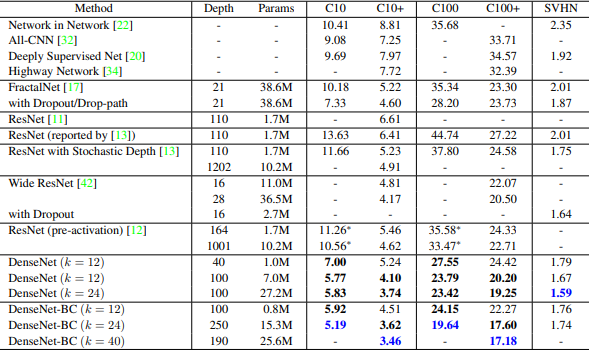
\includegraphics[width=1\linewidth]{images/selected_model}
	\caption{Tỉ lể lỗi trên tập dữ liệu CIFAR và SVHN của các mô hình CNN.}
	\label{fig:selected_model}
\end{figure}

Chính vì những cơ sở trên, học viên quyết định sử dụng mô hình DenseNet cho phần mềm thử nghiệm của luận văn.

\subsection{Phân tích mô hình hệ thống}
Hệ thống chương trình thử nghiệm Phần mềm chuẩn đoán bệnh lao được thiết kế theo kiến trúc Client/Server năm tầng (hình \ref{fig:client_server_ntang}), trong đó:
\begin{itemize}
	\item {\bf Tầng thứ nhất} là tầng giao diện người phân loại, cụ thể là ứng dụng client trên trình duyệt, quản lý tương tác người phân loại với ứng dụng như chọn ảnh gửi lên server… và hiển thị kết quả phân loại do server gửi về.
	\item {\bf Tầng thứ hai} là tầng server quản lý cấu hình hệ thống, ví dụ cấu hình giao thức gửi/nhận dữ liệu với client, cụ thể giao thức được sử dụng trong hệ thống là giao thức HTTP.
	\item {\bf Tầng thứ ba} là tầng server thực hiện logic xử lý các yêu cầu từ client, như	quản lý và phân phối các luồng xử lý độc lập, đảm bảo hiệu năng và chất lượng tính toán phân loại cho nhiều client trong cùng một thời điểm.
	\item {\bf Tầng thứ tư} là tầng đảm nhiệm xây dựng, tinh chỉnh và quản lý các phiên	bản mô hình phân loại cho hệ thống, với bộ ảnh huấn luyện được lấy từ tầng quản lý dữ liệu bên dưới.
	\item {\bf Tầng cuối cùng} là tầng quản lý dữ liệu, bao gồm CSDL ảnh phục vụ cho việc huấn luyện mô hình, CSDL ảnh đã xử lý từ các client nhằm mục đích bổ sung sự	đa dạng của CSDL ảnh và cải thiện độ chính xác của mô hình phân loại. Các bộ ảnh trên được lưu tách biệt để thuận tiện cho việc quản lý và đánh giá độ chính xác của các
	phiên bản mô hình huấn luyện cũng như mức độ ảnh hưởng của bộ ảnh huấn luyện lên chất lượng mô hình.
\end{itemize}
\begin{figure}[H]
	\centering
	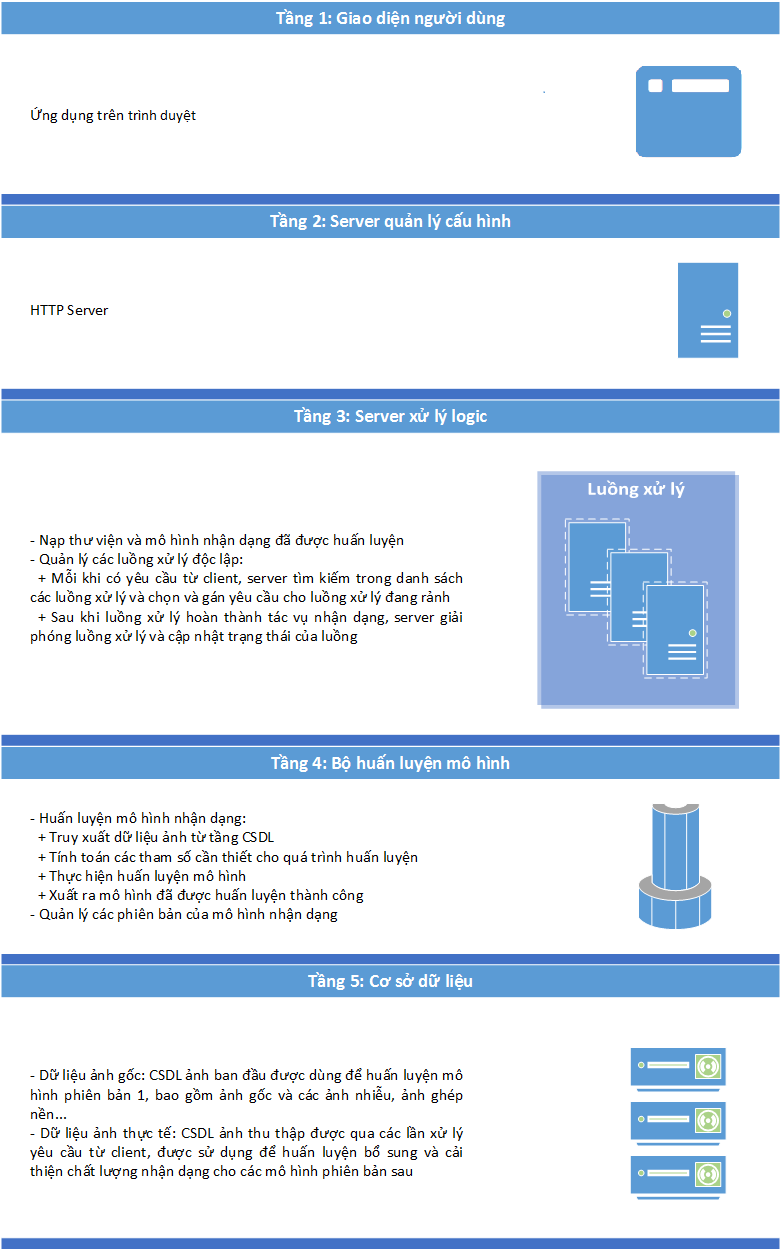
\includegraphics[width=1\linewidth]{images/client_server_ntang}
	\caption{Kiến trúc Client/Server năm tầng.}
	\label{fig:client_server_ntang}
\end{figure}

Luồng hoạt động chính của hệ thống được thể hiện trong hình \ref{fig:app_sequence}, trong đó các bước thực hiện của server và client từ lúc khởi động ban đầu tới lúc kết thúc như sau:
\begin{itemize}
	\item Client (ứng dụng trên trình duyệt)
	\begin{enumerate}
		\item Người phân loại khởi động ứng dụng/website.
		\item Người phân loại thực hiện chọn ảnh chụp x-quang trước đó được lưu trong máy tính để gửi.
		\item Ảnh chụp được mã hóa, nén lại và gửi tới máy chủ.
		\item Ứng dụng đợi nhận kết quả phân loại từ máy chủ gửi về và hiển thị cho người phân loại
	\end{enumerate}
	\item Chương trình Server
	\begin{enumerate}
		\item Chương trình được khởi động và nạp các thư viện cần thiết.
		\item Chương trình nạp mô hình phân loại đã được huấn luyện trước đó.
		\item Giao thức gửi, nhận dữ liệu giữa ứng dụng phía client và chương trình server được cấu hình.
		\item Một loại các luồng xử lý được khởi tạo, đặt trạng thái ban đầu là trạng thái sẵn sàng.
		\item Khi có ứng dụng client kết nối tới, chương trình kiểm tra trong danh sách các luồng xử lý và chọn một luồng đang ở trạng thái sẵn sàng để nhận và tính toán dữ liệu do client gửi tới.
		\item Trong luồng xử lý:
		\begin{itemize}
			\item Bắt đầu quá trình tính toán phân loại, cờ trạng thái là “bận”.
			\item Thực hiện giải nén dữ liệu thành dữ liệu ảnh gốc.
			\item Sử dụng mô hình đã nạp để phân loại ảnh.
			\item Trả kết quả phân loại về cho ứng dụng client.
			\item Kết thúc quá trình tính toán.
		\end{itemize}
		\item Khi luồng xử lý đã hoàn thành quá trình tính toán phân loại, chương trình giải phóng luồng xử lý bằng cách cập nhật lại trạng thái hiện tại của luồng.
	\end{enumerate}
\end{itemize}
\begin{figure}[H]
	\centering
	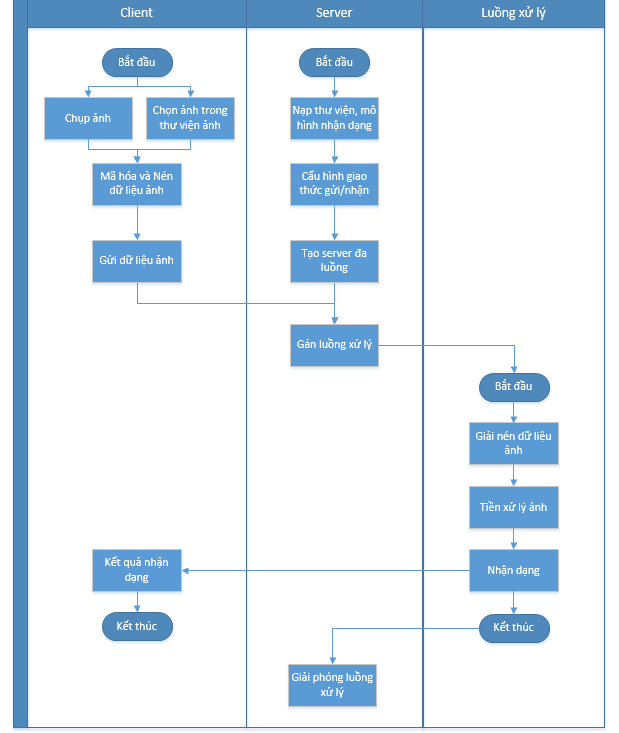
\includegraphics[width=1\linewidth]{images/app_sequence}
	\caption{Luồng hoạt động chính của hệ thống.}
	\label{fig:app_sequence}
\end{figure}

\section{Một số kết quả chương trình}
\subsection{Một số giao diện và chức năng chính chính của chương trình}
\subsection{Giao diện đăng nhập hệ thống}
Giao diện đăng nhập hệ thống cung cấp lớp bảo vệ cơ bản cùng khả năng định danh người dùng, từ đó đưa ra nhưng ngữ cảnh thực đơn phù hợp.
\begin{figure}[H]
	\centering
	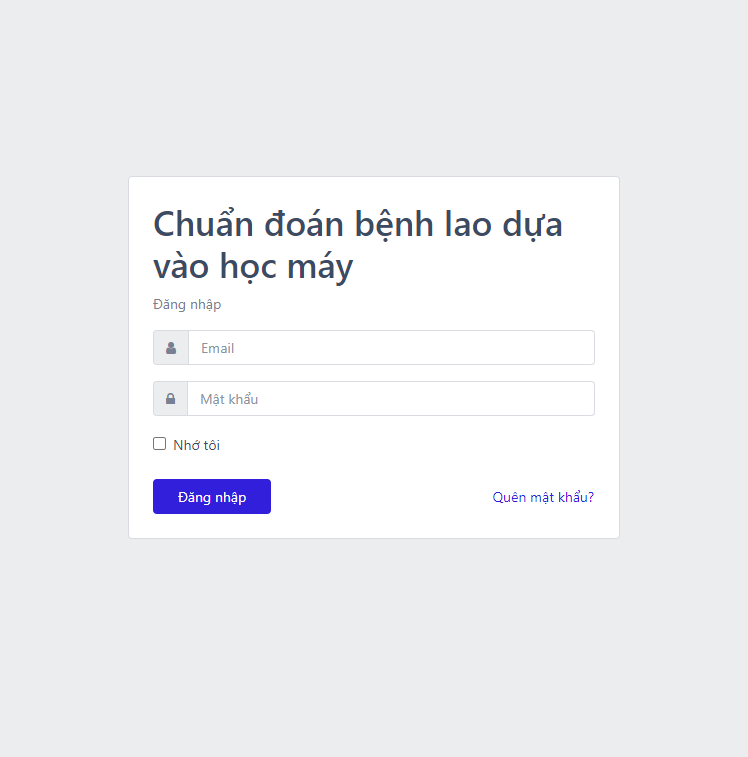
\includegraphics[width=1\linewidth]{images/giaodien_dangnhap}
	\caption{Giao diện đăng nhập hệ thống.}
	\label{fig:giaodien_dangnhap}
\end{figure}

\subsubsection{Giao diện cập nhật mô hình}
Tại đây, quản trị viên có thể thay đổi mô hình được sử dụng trong hệ thống. Mô hình này là được tạo ra ở pha Học. Mô hình mới được tải lên server, lưu trữ lại và ghi lại thông tin về đường dẫn để hệ thống có thể gọi được khi cần thiết.
\begin{figure}[H]
	\centering
	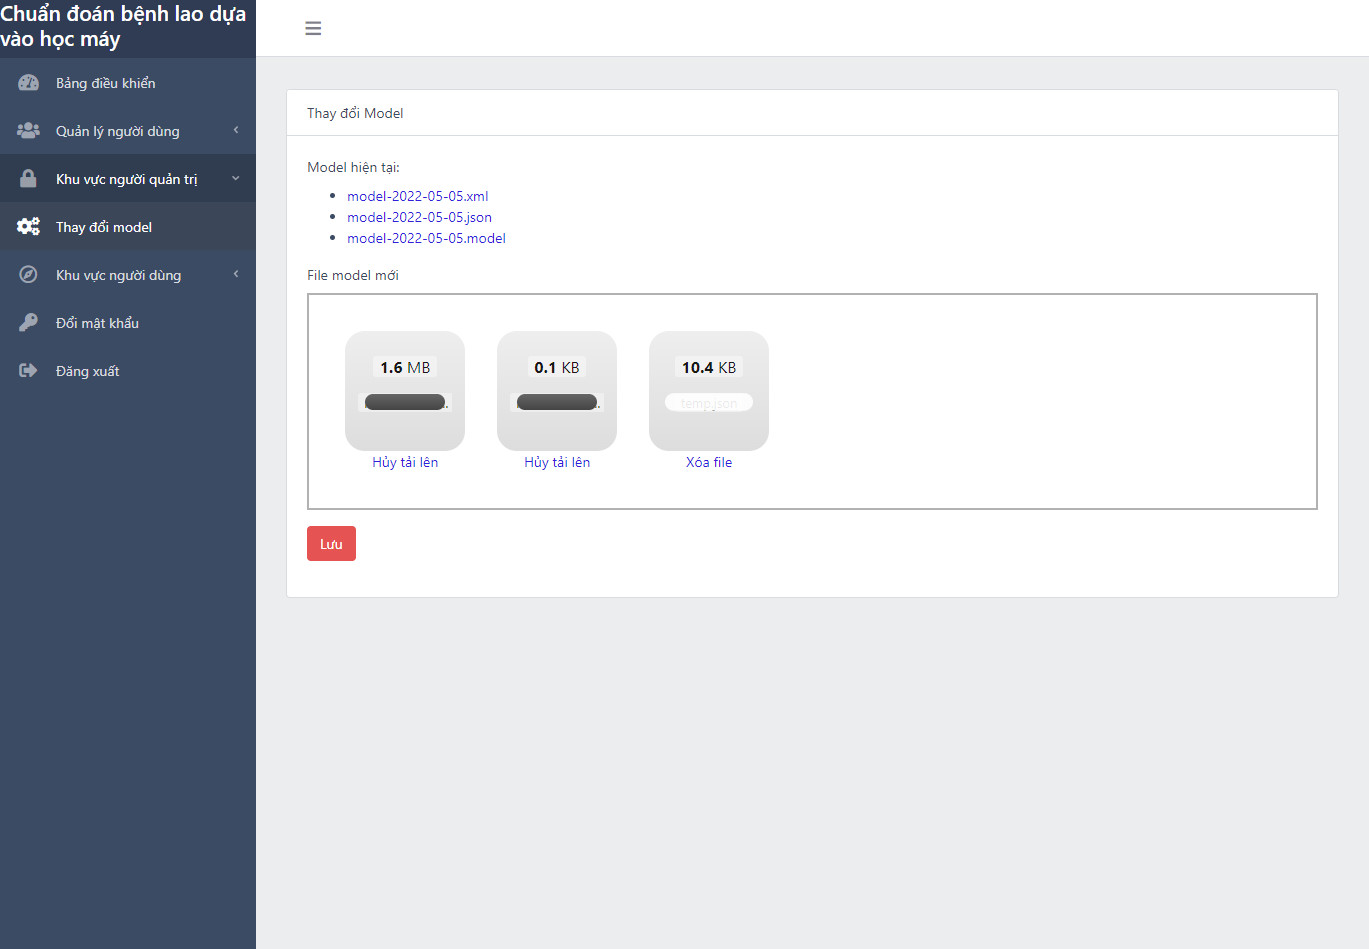
\includegraphics[width=1\linewidth]{images/quantri_doi_model}
	\caption{Giao diện cập nhật mô hình được sử dụng của hệ thống.}
	\label{fig:quantri_doi_model}
\end{figure}

\subsubsection{Giao diện danh sách các dự đoán}
Giao diện này tập trung thông tin của tất cả các dự đoán đã được thực hiện và lưu lại của hệ thống. Hệ thống sẽ hiện thị tất cả các dự đoán đối với người quản trị, và với tài khoản người dùng, hệ thống chỉ hiển thị những dự đoán thuộc về người dùng.
\begin{figure}[H]
	\centering
	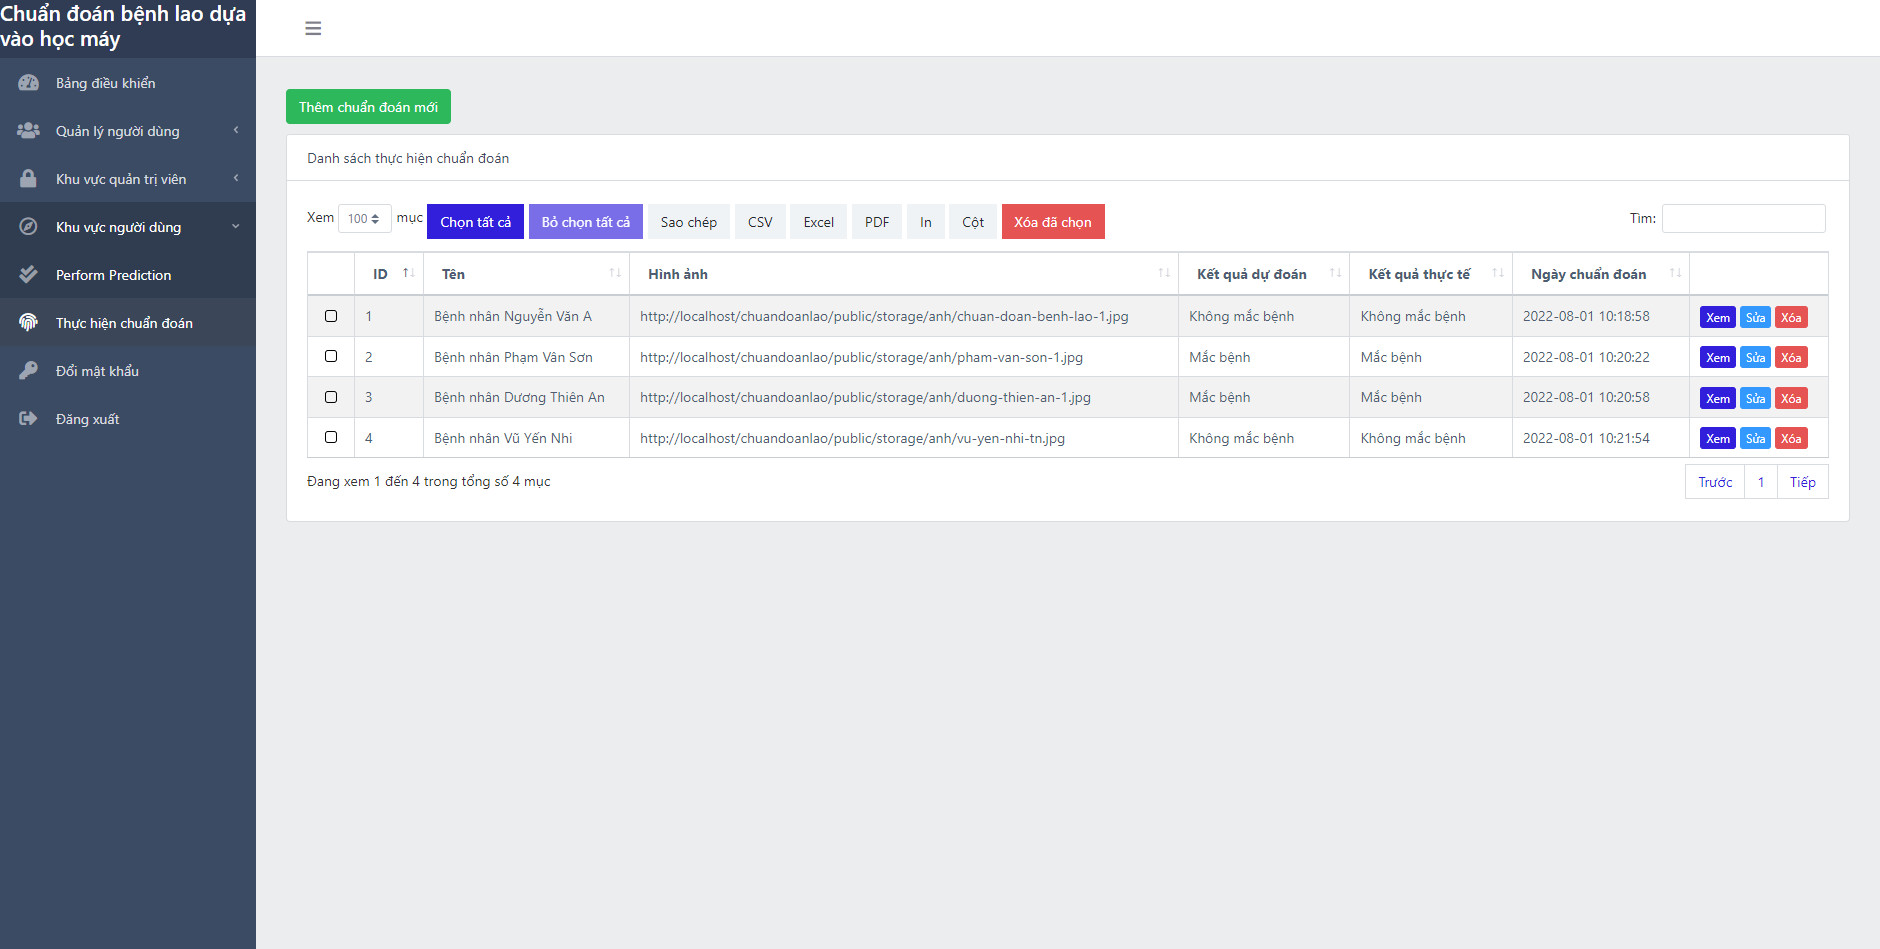
\includegraphics[width=0.95\linewidth]{images/user_danh_sach}
	\caption{Giao diện danh sách các dự đoán của hệ thống.}
	\label{fig:user_danh_sach}
\end{figure}

\subsection{Giao diện thực hiện dự đoán}
Người dùng upload ảnh chụp x-quang đã chuyển đổi định dạng PNG với kích thước 512x512 tại đây và nhận về kết quả dự đoán.
\begin{figure}[H]
	\centering
	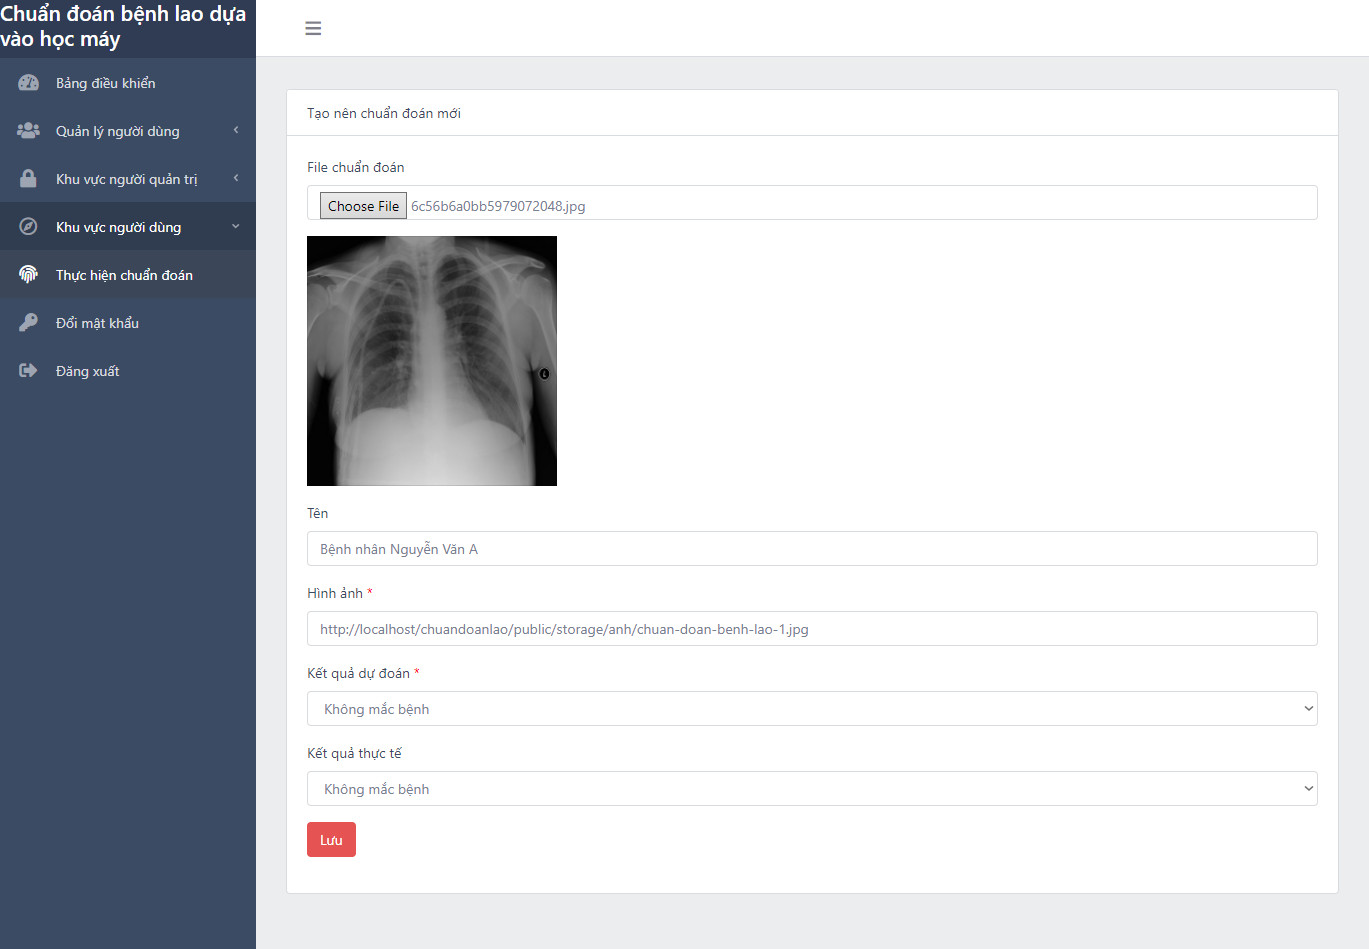
\includegraphics[width=0.95\linewidth]{images/user_du_doan_chi_tiet}
	\caption{Giao diện thực hiện phân loại của hệ thống.}
	\label{fig:user_danh_sach}
\end{figure}

\subsection{Một số ca phân loại được thực hiện bởi chương trình}
Thực hiện kiểm thử việc phân loại của hệ thống với 100 ảnh x-quang được tách riêng biệt khỏi quá trình trainning, ta có được kết quả rất khả quan.
\begin{figure}[H]
	\centering
	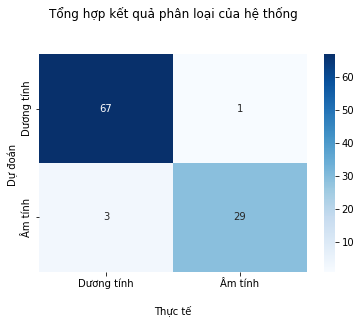
\includegraphics[width=0.66\linewidth]{images/result_backtest}
	\caption{Tổng hợp các ca phân loại của hệ thống.}
	\label{fig:result_backtest}
\end{figure}
Bài toán của luận văn chỉ có hai lớp để phân loại nên phương pháp thích hợp nhất để đánh giá là True/False Positive/Negative. Ta định nghĩa lớp dữ liệu quan trọng hơn cần được xác định đúng là lớp Positive (P-dương tính), lớp còn lại được gọi là Negative (N-âm tính). Ta định nghĩa True Positive (TP), False Positive (FP), True Negative (TN), False Negative (FN) dựa trên confusion matrix chưa chuẩn hoá. 

Bằng phương pháp trên, ta có kết quả tổng hợp tại hình \ref{fig:result_backtest}, tỉ lệ dự đoán chính xác là 96\%, tỉ lệ báo động nhầm (False Alarm Rate) là 1\% và tỉ lệ bỏ sót (Miss Detection Rate) là 3\%.  
